\section{Overview of Lorentz transformations and 4-vectors}
\label{sec:ltqs}
\subsection{Notation}
\[ x = (x^0, x^1, x^2, x^3) = (ct, x, y, z)\]
%  while $\vec{x}$ represents the space components only:
\[
\vec{x} = (x^1, x^2, x^3) = (x, y, z)
\]
Note that the symbol $x$ can refer to the four vector $x=(ct, x, y, z)$, as well as the first spatial component $x=x^1$. This has to be deduced from the context.
\subsection{Lorentz transformations}
Lorentz transformations transform between two frames that have a constants velocity relative to each other. They includes rotations, shifts and boosts.
The transformation for a boost in $x$ direction (with $\beta = v/c, \gamma = \frac{1}{\sqrt{1-\beta^2}}$) is given by:
\begin{equation}
\vIV{ct^{\prime}}{x^{\prime}}{y^{\prime}}{z^{\prime}}= 
      \left( \begin{array}{cccc} \gamma       & -\beta\gamma &  0  & 0  \\ 
                                 -\beta\gamma &  \gamma      &  0  & 0  \\
                                        0     &    0         &  1  & 0  \\
                                        0     &    0         &  0  & 1
             \end{array} \right)\vIV{ct}{x}{y}{z} 
\end{equation}
and in the y-direction
\begin{equation}
\vIV{ct^{\prime}}{x^{\prime}}{y^{\prime}}{z^{\prime}}= 
      \left( \begin{array}{cccc} \gamma       &   0 & -\beta\gamma &  0  \\ 
                                     0        &   1 &   0 & 0  \\
                                 -\beta\gamma &   0 & \gamma     & 0  \\
                                        0     &    0         &  0  & 1

             \end{array} \right)\vIV{ct}{x}{y}{z} 
\end{equation}
and in the z-direction
\begin{equation}
\vIV{ct^{\prime}}{x^{\prime}}{y^{\prime}}{z^{\prime}}= 
      \left( \begin{array}{cccc} \gamma       &   0 & 0 & -\beta\gamma  \\ 
                                     0        &   1 & 0 & 0  \\
                                     0        &   0 & 1 & 0  \\
                                 -\beta\gamma &   0 & 0  & \gamma
             \end{array} \right)\vIV{ct}{x}{y}{z} 
\end{equation}
Note that rotations are also a kind of Lorentz transformation, but one that only affects the space component. Below a rotation about the $z$ axis:
\begin{equation}
\vIV{ct^{\prime}}{x^{\prime}}{y^{\prime}}{z^{\prime}}= 
      \left( \begin{array}{cccc}      1     &  0 &  0  & 0  \\ 
                                0     &  \cos\theta  &  \sin\theta  & 0  \\
                                0     &  -\sin\theta & \cos\theta  & 0  \\
                                0     &    0         &  0  & 1
             \end{array} \right)\vIV{ct}{x}{y}{z} 
\end{equation}
A general Lorentz transformation is a combination of rotations, boosts, and co-ordinate shifts as in $x' = x + \delta x$.

\subsection{Four Vectors}
Four-vectors are defined as objects that transform under Lorentz transformations like  $(c\mathit{\Delta t}, \mathit{\Delta x}, \mathit{\Delta y}, \mathit{\Delta z})$, i.e. differences in $ct, x, y, z$. The most important four-vectors are:
\begin{align}
  \Delta x &= \vIV{c\Delta t}{\Delta x}{\Delta y}{\Delta z}
& dx &= \vIV{c\,dt}{dx}{dy}{dz}
& p &= \vIV{E}{cp_x}{cp_y}{cp_z}
& \partial &= \vIV{\partdbyd{}{(ct)}}{-\partdbyd{}{x}}{-\partdbyd{}{y}}{-\partdbyd{}{z}}
\end{align}
If we consider only rotations and boosts ("proper" Lorentz transformations), and not shifts (like $x' = x + \delta x$), then (ct, x, y, z) also transforms like a 4-vector.

The above leads to the following important relationships:
\begin{align}
\label{eq:EandP_fromBetaGammaM}
E &= \gamma m c^2 & \left|\vec{p}\right| = \beta \gamma m c
\end{align}
where $\beta$ is the speed of the particle, and $\gamma = 1/\sqrt{1-\beta^2}$
Note: In these notes, $m$ always refers to the rest mass of a particle, in some books called $m_0$. We do not use the concept of a speed-dependent mass $m_{\mathrm{some\;other\;books}}=\gamma m$, instead we write out the $\gamma$ factor explicitly as in $E=\gamma mc^2$.
\\\exercise{
Derive equation~\ref{eq:EandP_fromBetaGammaM} from $E=mc^2$ for a particle at rest.
\vspace{1ex}\\
\rotatebox{180}{\parbox{0.9\textwidth}{Answer: Without loss of generality we can pick a coordinate system where $\vec{p} = (p_x, 0, 0)$, and the particle moves with speed $v_x$. Boosting from the system where the particle is at rest to our system corresponds to a boost of $-\beta_x = -v_x/c$ (note the $-$ sign). Then
\begin{equation*}
      \left( \begin{array}{cccc} \gamma       &  \beta_x\gamma &  0  & 0  \\ 
                                 \beta_x\gamma &  \gamma      &  0  & 0  \\
                                        0     &    0         &  1  & 0  \\
                                        0     &    0         &  0  & 1
             \end{array} \right)\vIV{mc^2}{0}{0}{0} 
= \vIV{\gamma mc^2}{\beta_x\gamma mc^2}{0}{0} 
\end{equation*}
So $E = \gamma mc^2$ and $|\vec{p}| = p_x = \beta_x\gamma mc^2 / c = \beta_x\gamma mc $.}}
}
\\\exercise{What's the speed of a particle with energy $E=\un{1}{GeV}$ and momentum $\vec{p} = (0, 0, \un{0.9}{GeV}/c)$?
\rotatebox{180}{Answer: $v = 0.9c$}
}
\subsection{Invariants and dot products}
Dot products between four vectors are defined like this
\begin{equation}
A \cdot B = A^0 B^0 - \vec{A} \cdot \vec{B}
\end{equation}
are Lorentz invariant, i.e. they are the same in any coordinate system. This also works for $A \cdot A$, giving for each four vector $A$ one invariant $A^2$.
Especially important is
\begin{equation}
s = p^2 = p \cdot p = E^2 - c^2 \vec{p}^2
\end{equation}
In the centre of mass frame, $\vec{p}=\vec{0}$, so we see that $\sqrt{s}=E_{cm}$, is the centre-of-mass energy. For an individual particle with momentum $p$, $p^2=(mc^2)^2$ where $m$ is the particle's mass. This is important enough to write down again:
\begin{align}
(mc^2)^2 &= E^2 - (pc)^2 &\mathrm{or}\; E^2 &= (mc^2)^2 + (pc)^2
\end{align}
Consider a particle moving a differential line element $d\vec{x}$ in time $dt$. The differential four interval
\begin{equation}
ds^2 \equiv dx\cdot dx = c^2dt^2 - \left|d\vec{x}\right|^2 = c^2dt^2 \left(1-\beta^2\right)
\end{equation}
is also an important invariant. (Beware of the potentially confusing re-use of the variable $s$ in this context.) In the rest frame of the particle, $d\vec{x}=0$, and we identify $ds$ with the differential of the proper time
\begin{equation}
 d\tau = dt \sqrt{1-\beta^2} = \frac{dt}{\gamma_u};
\label{eq:proptime}
\end{equation}
 $\tau$ is the proper time of the particle, which is the same as the time of the particle at rest. Time intervals observed from a moving co-ordinate
system are stretched by a factor of $\gamma$ relative to the time in
the restframe - the famous time dilation.
\\\exercise{
\begin{enumerate}
\item A particle  has energy $E=\un{1.118}{GeV}$ and momentum $\vec{p}=(0, 0, \un{1}{GeV/c})$. What is its mass?
\item The same particle is observed in reference frame $S'$ with momentum $\vec{p}'=(\un{0.5}{GeV/c}, \un{0.5}{GeV/c}, 0)$. What is its energy, now?
\item In frame $S'$, the particle exists for $\un{1}{fs}$ before it decays. How long did it exist in its own restframe? (Hint: use $E=\gamma m c^2$.)
\end{enumerate}
\rotatebox{180}{Answers: $m=\un{0.5}{GeV/c^2}$, $E'=\un{0.866}{GeV}$, $t_{\mathrm{rest}} = \un{0.577}{fs}$}
}

\section{Particle kinematics}
In Sec.~\ref{sec:ltqs} we discussed 4-momentum and how
it transform under a Lorentz-boost. One important point
is that energy and momentum conservation still applies. These
conservation rules are different to frame invariance, and rather
refer to conservation in time ie
\[
E_{\rm TOTAL}=E_{1}+E_{2}+...+E_{n}
\]
and 
\[
\vec{p}_{\rm TOTAL}=\vec{p}_{1}+\vec{p}_{2}+...+\vec{p}_{n},
\]
are both conserved quantities at any point in space and time.
However:
\[
m_{\rm TOTAL}=m_{1}+m_{2}+...+m_{n},
\]
is NOT conserved, but IS invariant under Lorentz transformations.

\noindent Let us consider a couple of applications of energy-momentum conservation
in particle collisions. In particle physics,
\noindent 
\[
m^{2}=p_{\rm TOTAL}\cdot p_{\rm TOTAL}=E^{2}_{\rm TOTAL}-\vec{p}^{2}_{\rm TOTAL},
\]

is used to quantify the energy involved in a collision. As $m^{2}$ is a Lorentz invariant quantity, 
it is equivalent to the total energy squared in a frame where $\vec{p}^{2}_{\rm TOTAL}=0$ 
i.e the Centre of Mass (CoM) frame. Therefore we can define $s\equiv m^2$ and  thus $\sqrt{s}$ is the CoM energy.

\paragraph{Example 1: ``Fixed target'' collision}
\begin{center}
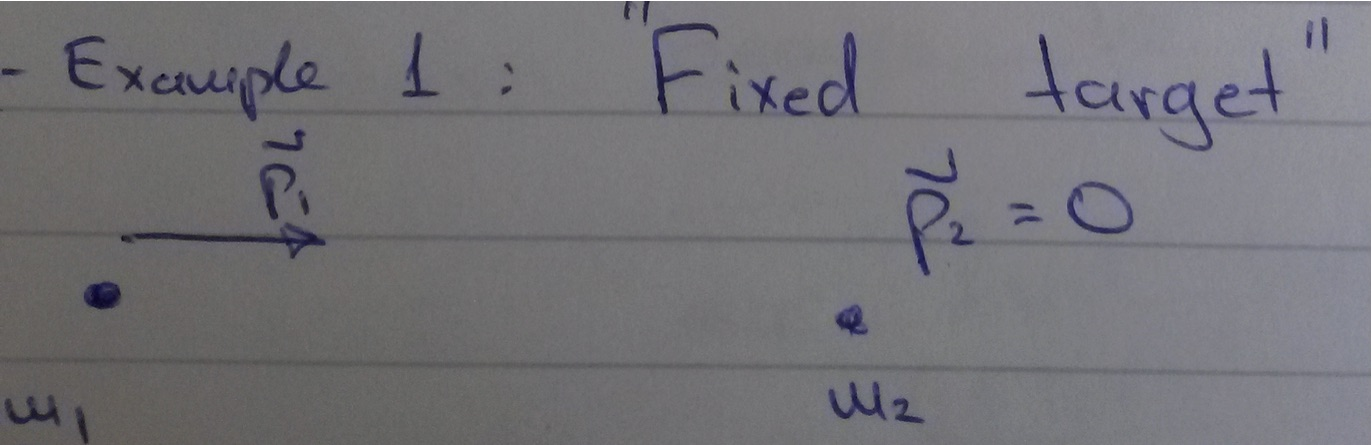
\includegraphics[width=0.5\textwidth]{fig/collisions/collisions_example1.jpg}
\end{center}

In this example
\[
s=(E_{1}+E_{2})^{2}-(\vec{p_1})^2.
\]
since $\vec{p_2}=\vec{0}$. Remembering 
that $|p_1|^2=E_{1}^{2}-m_{1}^{2}$ (using natural units) and rearranging, we get
\[
E_{1}=\frac{s-m_{1}^{2}-m_{2}^{2}}{2m_{2}}.
\]
\noindent Therefore in a fixed target collision, in order to achieve a CoM 
energy $\sqrt{s}$, one needs a beam of energy as given above.  If we make the assumption that the required $s$ is much larger than $m_{1}^2$ and $m_{2}^{2}$, then the expression for the beam energy of a fixed target collider reduces to\footnote{Particle beams
consist of electrons or protons or pions or kaons. All these particles have masses $<1$~GeV.
The mass of the target does not refer to the macroscopic mass of the whole target block, but rather to the microscopic mass of nucleus with which the proton interacts. For all practical purposes the mass of the target can be considered as the atomic mass of the nucleus. Depending on the target, the mass can vary between $\sim 1$~GeV for a hydrogen target to $\mathcal{O}(10)$~GeV for a beryllium target or $\mathcal{O}(100)$~GeV for a molybdenum target.}:
\begin{equation}
\label{eq:e_fixed_target}
E_{1}\sim \frac{s}{2m_{2}}.
\end{equation}

\paragraph{Example 2: ``Particle collider''}
\begin{center}
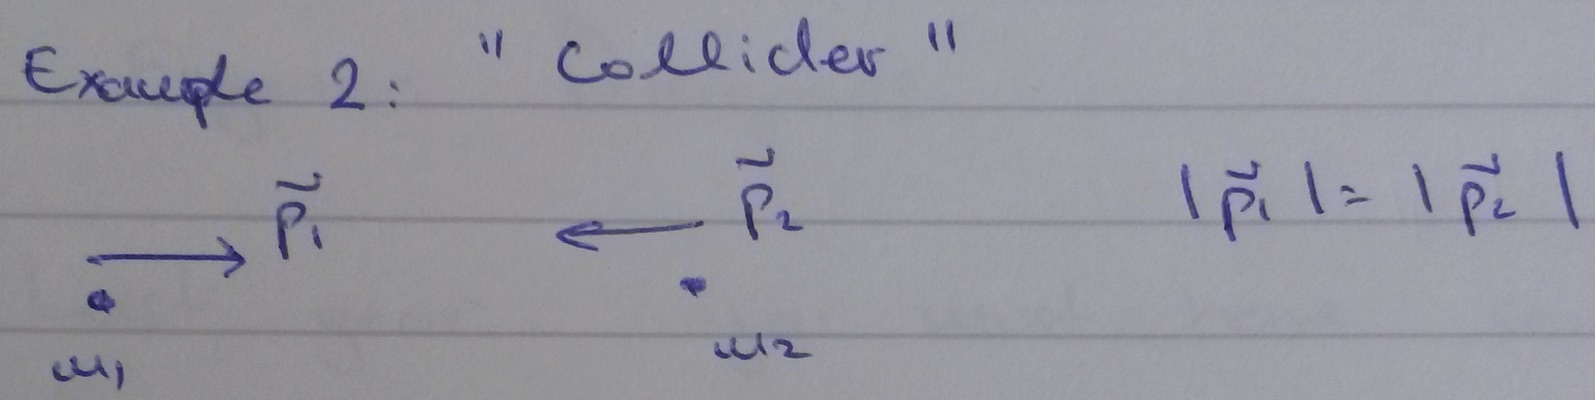
\includegraphics[width=0.5\textwidth]{fig/collisions/collisions_example2.jpg}
\end{center}
Consider two colliding beams with $\vec{p_1}=-\vec{p_2}$.
In this case:
\[
s=(E_{1}+E_{2})^{2}.
\]
Using  $|p_1|^2=|p_2|^2$ we have:
\[
E_{1}^{2}-E_{2}^{2}=m_{1}^{2}-m_{2}^{2}
\]
Therefore we can replace $E_2$ in favour of $E_1$ and get:
\[
E_1=\frac{s+m_{1}^{2}-m_{2}^{2}}{2\sqrt{s}}
\]
Under the assumption that $s \gg m_{1}^2,m_{2}^2$, we can write:
\begin{equation}
\label{eq:e_collider}
E_{1}\sim \frac{\sqrt{s}}{2}.
\end{equation}

Consider now that we want to build an accelarator which produces collisions
at $\sqrt{s}=13$000~GeV (13~TeV), very much like the Large Hadron Collider running
currently at CERN. Given Eq.~\ref{eq:e_collider}, one would require a beam energy of 6.5~TeV per beam. 

If however we were to use a ``fixed-target'' type facility, then using Eq.~\ref{eq:e_fixed_target}, where we consider a hydrogen target in which case $m_{2}\sim 1$~GeV, the required beam energy would be $E_{1}=\frac{13000^2}{2\times1}\sim84.5$~PeV!!

These two examples illustrate why if one is after high energies, it is much more efficient to accelerate and collide two beams rather than whack a single beam onto a target. If however one is interested in a large number of collisions (high intensity rather than high energy) then the most efficient way is a ``fixed target'' configuration.

\exercise{
When the Large Hadron Collider started colliding beams at $\sqrt{s}=13$~TeV, some members of the press claimed that: ``The Large Hadron Collider produces the highest energy collisions in our solar system ''. 

Cosmic rays are high energy charged particles originating outside our solar system. They have been observed to have energies up to $10^{20}$~eV. By considering the collision of the most energetic cosmic ray with stationary hydrogen gas in the universe decide whether the statement was correct.
\rotatebox{180}{Answer: Cosmic ray on Hydrogen $\sqrt{s}\sim450$~TeV.
%Hydrogen gas means the target particle is\\ a proton of mass $m_p\sim 1$~GeV. So for a fixed target collision we have $\sqrt{s}\sim\sqrt{2E m_p}$ Therefore $\sqrt{s}\sim\sqrt{1\times10^{20}\times1\times10^9}\sim450~$~TeV,\newline compared to LHC's 13~TeV so the statement was incorrect.
}
}

